\chapter{Methodology}
\label{ch:problem}

This chapter formally defines the POMDP used to model the shared-control lane-keeping task that is considered in this thesis. Furthermore, the chosen solution approach and how it was applied for the defined task are presented. Section \ref{sec:lane_keeping_loop} begins with an overview of the three components comprising the problem: The driver model representing the human driver, the driving simulator, and the agent assisting the driver. The simple driver model that we use to simulate human driving behavior is specified in section \ref{sec:driver_model}. Section \ref{torcs} describes how \acrfull{torcs} is used to simulate the dynamics of a car driving on a highway. The agent employs the \acrfull{pomcp} algorithm to solve the POMDP online. A detailed explanation of how the algorithm is applied is provided in section \ref{sec:pomcp}.

\section{Overview}

The problem addressed in this thesis is an assisted driving lane-keeping task, where a human driver shares control with an agent over a car. The driver and the agent cooperatively control the steering wheel. The goal is to keep the car centered in its lane. Both the agent and the driver have only lateral control; the car's speed is fixed. The driver can be attentive or distracted and alternates between the two states. The general assumption is that an attentive driver shows (nearly) optimal steering behavior, while a distracted driver steers suboptimally and needs assistance. The agent, however, cannot observe whether the driver is attentive or not. To fulfill the goal of consistently keeping the car centered in the lane, the agent has to effectively estimate the driver's state of attentiveness according to the information it receives over time. Based on its estimate, the agent determines what actions the driver is likely going to take. It can then plan ahead and select adequate steering actions.

\begin{figure}[htbp]
    \centerfloat
    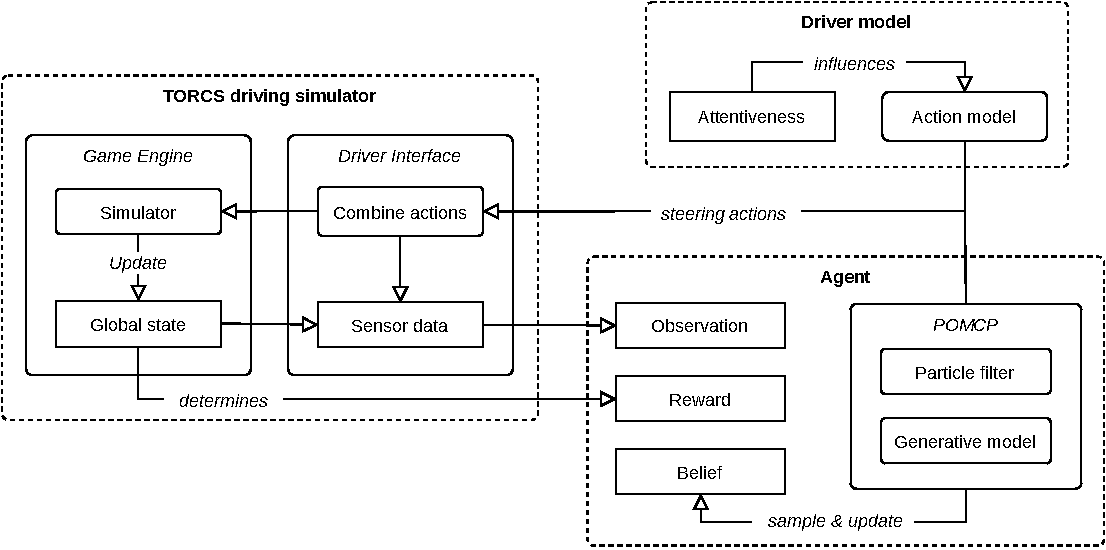
\includegraphics[width=1.0\textwidth]{figures/Components.pdf}
    \caption{Overview of the modules used to represent and solve the shared control lane keeping POMDP}
    \label{fig:overview}
\end{figure}

Rather than experimenting with real humans and a real car, simulation models are used for both the car and the human driver in experiments. Figure \ref{fig:overview} gives an overview of the three distinct modules employed to represent the problem as a POMDP and solve it: First, the racing car simulator TORCS \parencite{torcs} simulates the dynamics of a car driving on a highway. Second, the driver model substitutes the human driver. Third, the agent applies POMCP in order to solve the POMDP online. From the perspective of the agent, its environment is composed of both the simulated car and the simulated driver. The simulation modules are described in detail in the following subsections. 

\subsection{TORCS as a highway driving simulator}
\label{torcs}

\acrfull{torcs} is an open-source car driving simulator \parencite{torcs}. As the name suggests, TORCS was initially developed to simulate racing car tournaments. However, as racing cars are fundamentally also just cars and everything, including the tracks, is highly customizable, highway driving can be simulated just as well. Part of TORCS is a comprehensive and realistic discrete-time simulation engine to simulate car dynamics, as well as an \glsentryshort{api} for computer-controlled drivers, so-called robots. It has been widely used by researchers to simulate car driving and to evaluate the performance of autonomous driving agents (for example in \cite{torcs-3}, \cite{torcs-1}, \cite{torcs-2}, and \cite{reward1}).

We use TORCS as a simulator for car dynamics for two purposes. First, to simulate the dynamics of the car the agent and the driver share control over. This simulation is part of the environment of the agent. It represents the car in the real world and would be replaced by an actual car in a realistic setting. TORCS maintains the car's true state and updates it based on the combined steering action. Second, we use the simulation engine as a generative model (see section \ref{sec:gen_model}). The generative model is part of the agent, constituting the agent's model of the world. The agent uses it to sample state and observation transitions for the forward search performed during the online MCTS policy computation (planning).
 
\begin{figure}[htbp]
    \centerfloat
    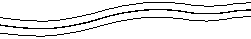
\includegraphics[width=1.0\textwidth]{figures/track.pdf}
    \caption{Course of the road of a section of the TORCS highway track used for experiments.}
    \label{fig:track}
\end{figure}

Typical racing tracks for TORCS have sharp road bends and wide roads with differing widths around the course. This does not reflect a highway driving scenario well. Therefore, a custom highway track is used instead (see figure \ref{fig:track}). The custom track only has moderate road bends and a constant lane width of 3.75m, as it is common in Europe \parencite{lane_width}. The road is completely flat and there are no other cars on it. Moreover, a fixed speed of 80 km/h is set during our experiments.

\subsection{Driver model}
\label{sec:driver_model}

In this study, the driver is simulated using a stochastic driver model, instead of performing experiments with an actual human driver. The driver model determines when a driver is attentive or becomes distracted, for how long the attentive or distracted period persists, and what actions the driver takes. We design a simple driver model to evaluate our approach. If the agent can plan successfully with a simple driver model, this serves as an initial confirmation that the solution approach is promising. The focus of this thesis is not a realistic driver model.

\subsubsection{Configurations}
\label{sec:driver_model_config}

Three different driver model configurations with increasingly complex dynamics are used in the experiments:
\begin{enumerate}
    \item \textbf{Simple driver model:} The simplest model steers optimally when the driver is attentive. If it is in a distracted state, the model repeats the last attentive steering action until the driver regains her attentiveness. A distracted driver's ability to notice changes in the course of the road is limited because of reduced situational awareness, and therefore she does not adjust to road changes like an attentive driver would (\cite{driver-awareness}; \cite{driver-awareness2}).
    \item \textbf{Steering overcorrection:} When a distracted driver diverts strongly from the lane center and then becomes attentive again, the driver suddenly notices the deviation. In this case, drivers tend to perform an overly strong steering correction and overshoot \parencite{oversteering-motivation}. We implemented this behavior in a second, more complex model. The first action of a driver that regains attentiveness is increased by a random amount between 10 and 25 percent. The randomness makes the model less predictable when the driver becomes attentive again.
    \item \textbf{Steering overcorrection and noise:} The last, most complex scenario introduces action noise. A random noise between five and 20 percent is added to every action the driver takes. The action can thereby become five to 20 percent stronger or weaker. The overcorrection for the first action after regaining attentiveness, introduced in the last model, is performed as well. The noise is added on top. The noise makes the driver less predictable in every situation.
\end{enumerate}


\section{Lane keeping with a human in the loop as a POMDP}
\label{sec:lane_keeping_loop}

In this section, we formulate the shared control lane-keeping problem as a POMDP. Refer to section \ref{sec:pomdp} for a general definition of a POMDP. In the following subsections, we define the state space and the state transition probabilities, the action space, the reward function, and the observation space with the observation probabilities. 

\subsection{States and transition probabilities}

The overall state space $S$ consists of all possible states of the agent's environment. For the agent, the environment is compiled of both the driver and the car. Therefore, the state space we have to consider in the POMDP is the combination of all possible combinations of the state of the car and the state of the driver model. The state transition probabilities $T$ are not explicitly given but implicitly defined by the car dynamics simulated by TORC's simulation engine.

\subsubsection*{Car state}
\label{sec:state}

TORCS data model for the car state is too extensive to list here in full\footnote{See \emph{tCar} struct in the \href{https://sourceforge.net/projects/torcs/files/api-docs/}{TORCS API documentation}}. Table \ref{tab:state} shows the most important attributes. These include the car's position on the track, its current velocity, and its acceleration. Among others, there are additional attributes for the state of transmission and engine, the friction and spin of the wheels, and aerodynamic influences such as drag and lift. The values in the state are continuous. 

\begin{table}[htbp]
\footnotesize
\centering
\centerfloat
\begin{tabular}{@{}ccccc@{}}
\toprule
\textbf{Long. position} & \textbf{Lat. position} &  \textbf{Yaw angle} & \textbf{Velocity}    & \textbf{Acceleration} \\ \midrule
115m (from start)              & 0 (lane center) & 45\textdegree           & 80 km/h (fixed)      & 0.3                   \\ \bottomrule 
\multicolumn{1}{l}{}           & \multicolumn{1}{l}{}      & \multicolumn{1}{l}{} & \multicolumn{1}{l}{}  \\ \toprule
\textbf{Transmission}          & \textbf{Engine}           & \textbf{Wheels}      & \textbf{Aerodynamics} & \textbf{...} \\ \midrule
gear, clutch, ...              & rpm, pressure, ...        & friction, spin, ...  & drag, lift, ...    & ...   \\ \bottomrule                                                                
\end{tabular}
\caption[Examplary car state]{Examplary car state. This is an incomplete table, only listing the most important attributes. For a full state representation, look up the \emph{tCar} struct in the \href{https://sourceforge.net/projects/torcs/files/api-docs/}{TORCS API documentation}.}
\label{tab:state}
\end{table}

\noindent
The lateral position (lane centeredness) and the yaw angle of the car are illustrated in figure \ref{fig:observations}. The lane centeredness of the car is defined over a continuous interval of $(-\infty,\infty)$, with values in between -1 (right lane border) and +1 (left lane border) denoting that the car is within its lane, and everything beyond standing for an off-track position. A value of zero means the car is centered in its lane. The car's relative yaw angle is given with respect to the track direction and defined over an interval of $[-\pi, +\pi]$ radians. A value of zero indicates that the car is heading in the same position as the track.

\begin{figure}[htbp]
    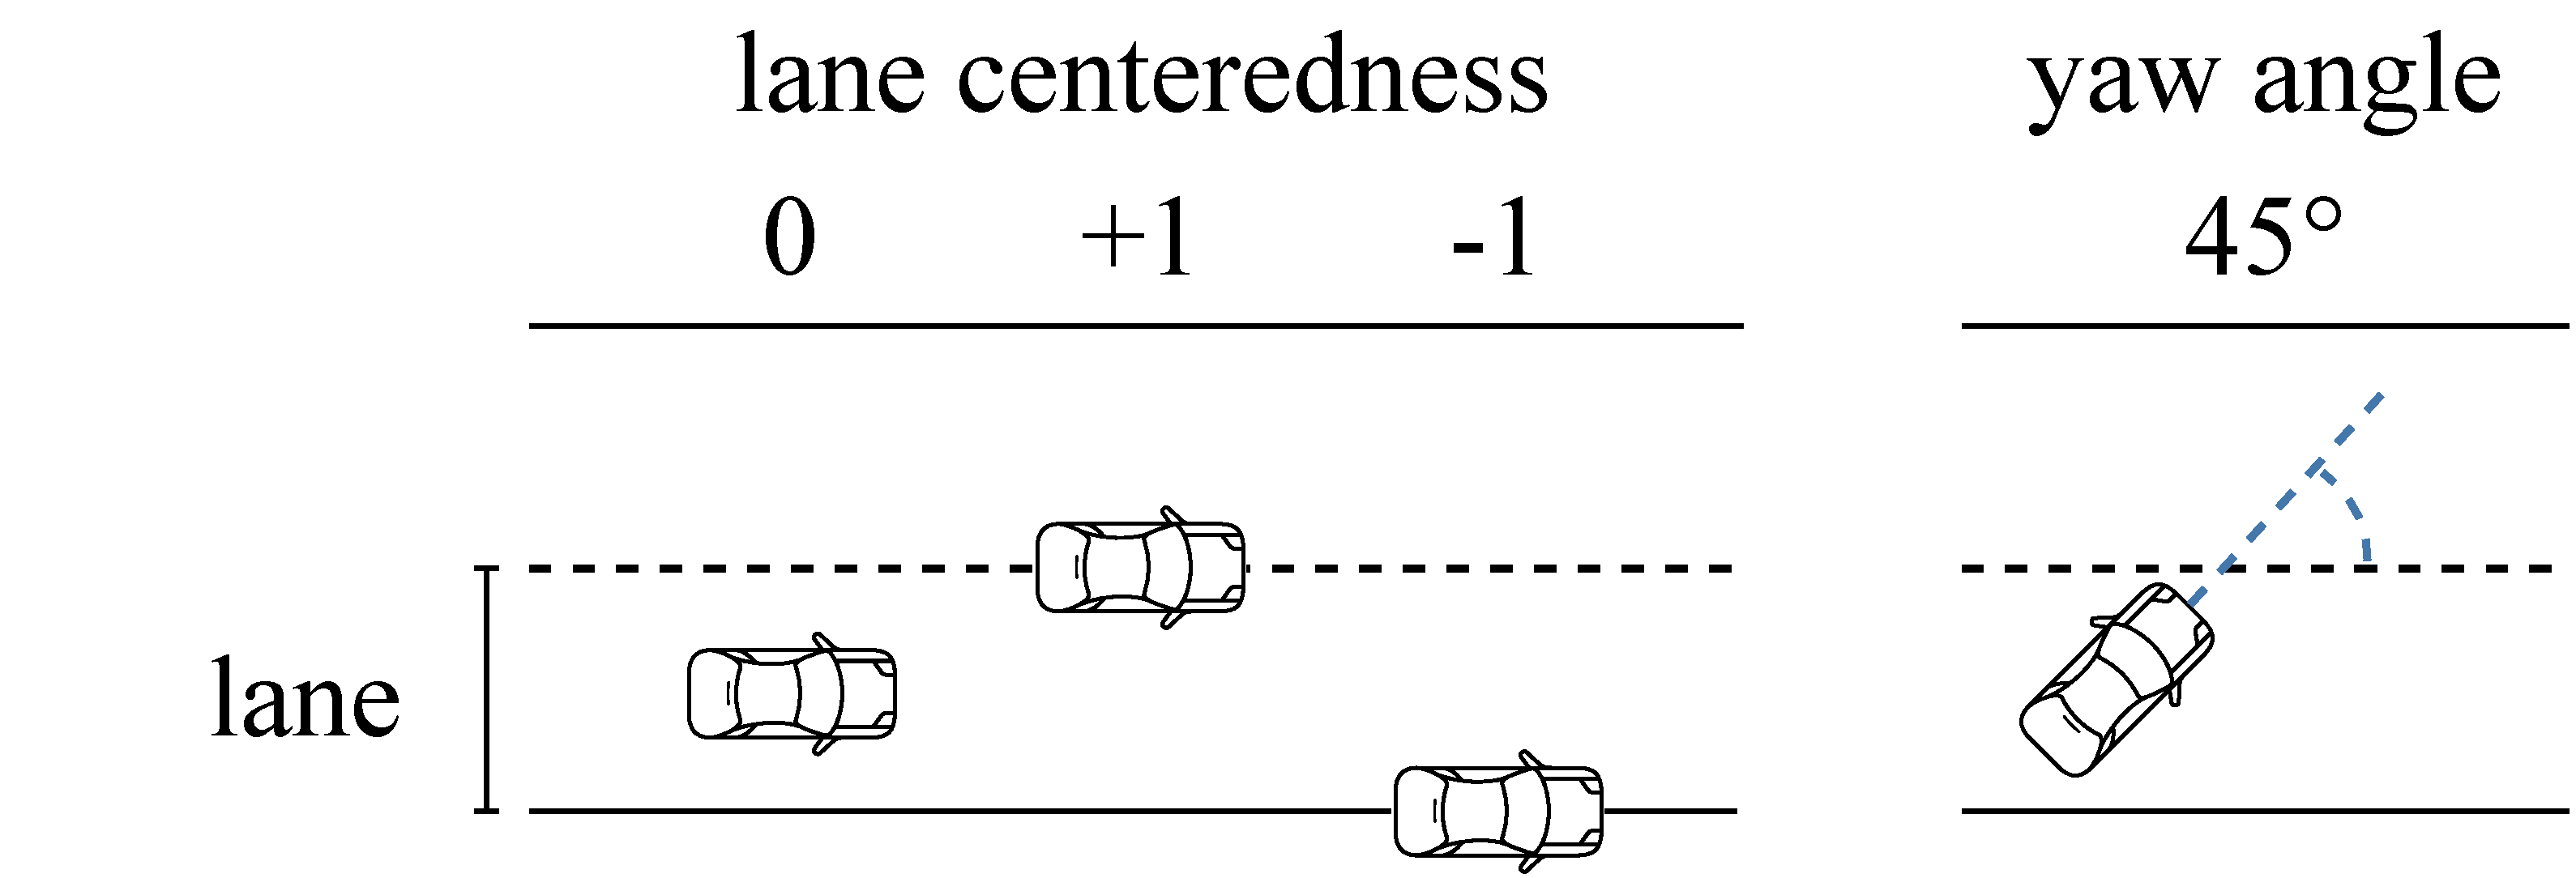
\includegraphics[width=0.6\linewidth]{figures/angle_distance.pdf}
    \centering
    \caption{Illustration of lane centeredness and yaw angle values}
    \label{fig:observations}
\end{figure}

\subsubsection*{Driver state}
\label{sec:driver_state}
The driver state consists of two variables: The current state (attentive or distracted) and the duration it remains in this current state. The duration it remains in a state is randomly chosen but lies between one second (10 actions) and 5 seconds (50 actions). When the time runs out for the current state, the state reverses; an attentive driver becomes distracted, and a distracted driver regains attentiveness. The duration for the next state is randomly chosen again. The process repeats until the experiment is over.

\subsection{Actions}
\label{sec:actions}

The action space $A$ consists of all steering actions \emph{the agent} can perform. In the experiments, two different sets of actions are referred to: First, a full action set, which enables the agent to overrule and effectively reverse the driver's actions completely. Second, a reduced action set containing only moderate steering actions (reduced action space in table \ref{tab:actions}). The motivation behind this is the assumption that strong steering actions are seldomly needed while driving on a highway. Leaving them away might reduce the planning complexity.

The human driver and the agent share control of the steering wheel. The steering input of the driver $a_{driver}$ and agent $a_{agent}$ are added to $a_{car} \in [-1, +1]$ using Equation~\ref{eq:steering}.

\begin{equation}
    a_{car} = \min(\, -1, \, \max(\, 1, \, (a_{driver} + a_{agent})\,)\,)
    \label{eq:steering}
\end{equation}

A steering action of $-1$ means steering fully to the right (159 degrees), and an action of $+1$ has the effect of fully steering to the left (21 degrees). The relationship between steering actions and steering angles is illustrated in figure~\ref{fig:steer-angle}.

\begin{figure}[htbp]
    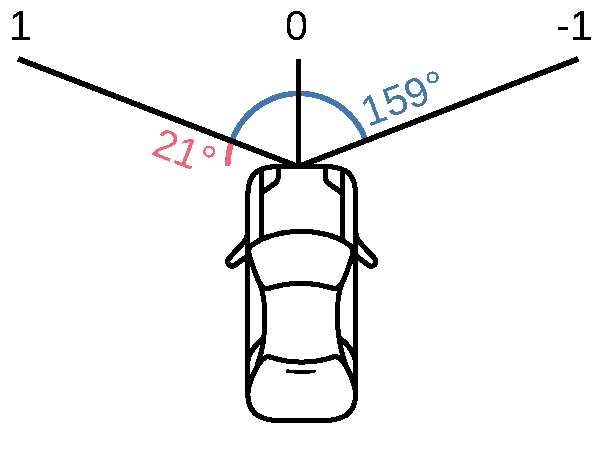
\includegraphics[width=0.3\linewidth]{figures/steering-angle.pdf}
    \centering
    \caption{Mapping steering actions to steering angles}
    \label{fig:steer-angle}
\end{figure}

\vspace{1em}
\noindent
Table \ref{tab:actions} shows the discrete actions for the driver and the agent. The discrete values have been chosen empirically. More actions allow for more precise control. However, the number of actions is the branching factor for the search tree construction during planning. Thus, it has a strong impact on the complexity of the search problem. Therefore, a compromise between precision and performance is made. Because minor actions are more likely and generally preferable in a highway driving scenario, the resolution is higher for small steering actions.

If the driver is distracted while the car is in a road bend, in the most extreme situation, she could potentially steer into the opposite direction of where she needs to steer to keep the car centered in its lane. In this case, to correct the driver's incorrect action, the agent needs to be able to effectively reverse the driver's action. Therefore, the action space of the agent is extended by plus two and minus two.

\begin{table}[htbp]
\footnotesize
\centering
\centerfloat
\setlength{\tabcolsep}{5pt}
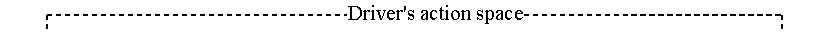
\includegraphics[width=0.925\textwidth]{figures/driver-actions.pdf}
\begin{tabular}{cccccccccccccccc}
\toprule
 -2 & -1     & -0.75  & -0.5   & -0.25  & -0.15  & -0.1   & 0     & 0.1   & 0.15  & 0.25  & 0.5   & 0.75  & 1 & 2 \\ \bottomrule
\end{tabular}
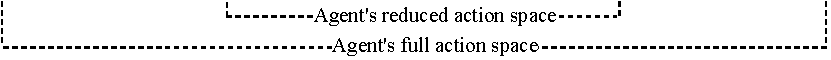
\includegraphics[width=0.925\textwidth]{figures/agent-actions.pdf}
\caption[Discrete steering actions for the driver and the agent]{Discrete steering actions for the driver and the agent.}
\label{tab:actions}
\end{table} 

\label{sec:driver_act_discr}
\noindent
The actions of the driver are naturally continuous. We discretize them by mapping their continuous values to the closest value in the discrete action space, as it can be seen in table \ref{tab:action_dist}.

\begin{table}[htbp]
\footnotesize
\centering
\centerfloat
\setlength{\tabcolsep}{3pt}
\begin{tabular}{@{}lccccccccccccc@{}}
\toprule
Action & -1     & -0.75  & -0.5   & -0.25  & -0.15  & -0.1   & 0     & 0.1   & 0.15  & 0.25  & 0.5   & 0.75  & 1 \\ \midrule
From   & -1   & -0.875 & -0.625 & -0.375 & -0.2   & -0.125 & -0.05 & 0.05  & 0.125 & 0.2   & 0.375 & 0.625 & 0.875 \\ 
To     & -0.875 & -0.625 & -0.375 & -0.2   & -0.125 & -0.05  & 0.05  & 0.125 & 0.2   & 0.375 & 0.625 & 0.875 & 1  \\ \bottomrule
\end{tabular}

% TODO: Fix caption!
\caption[Driver action discretization]{Driver action discretization. For negative values, the \emph{To} value is exclusive. For zero, both \emph{From} and \emph{To} are inclusive. For positive values, the \emph{From} value is exclusive.}
\label{tab:action_dist}
\end{table} 

\subsection{Reward}

The reward function $R$ is based on the car's distance to the center of the lane and its relative angle to the road path (see section \ref{sec:reward}). The attentiveness of the driver is not considered. The agent is expected to estimate it based on the driver's behavior alone. However, the reward is correlated with the quality of the agent's estimate as its actions can only lead to optimal steering behavior with a correct estimate.

\label{sec:reward}

The reward function defines the goal of the agent. For the task of lane centering, two sub-goals need to be considered: First, the car is supposed to stay as close to the lane center as possible. Second, the car's yaw angle (the direction into which the car is headed) should be as close to the track axis angle as possible. 

Equation \ref{eq:reward} shows the reward function for the agent that incorporates both targets. The relative yaw angle is denoted as $\theta$, and $\phi$ represents the lane centeredness (see figure \ref{fig:observations}). A lane centeredness of zero means the car is centered. If the car is on the left-most side of the lane, the value equals one. For the right-most side, it equals minus one. The agent receives the maximum reward if the car is in the middle of the road, while its relative yaw angle is equal to zero. Similar reward formulations have been used successfully before (\cite{reward1}; \cite{reward2}). The attentiveness of the driver is not directly included in the reward function. However, it is implicitly considered. If the agent performs an action that leads to a suboptimal combined steering action, it is penalized by receiving a lower reward. Thereby, if the agent acts when the attentive driver behaves optimally, it is punished indirectly.

\begin{equation}
    \label{eq:reward}
    R = 
    \begin{cases}
        \cos \theta + |\phi|,& \text{if } \phi \in [-1,+1]\\
        0,              & \text{otherwise}
    \end{cases}
\end{equation}

\subsection{Observations and observation probabilities}
\label{sec:observations}

\begin{table}[htbp]
\centering
\footnotesize
\begin{tabularx}{\textwidth}{p{0.20\textwidth}X}
\toprule
\textbf{Observation}& \textbf{Description and values}   \\ \midrule
Relative yaw angle          &  Angle between car direction and track axis direction. The continuous values between $-\pi$ and $\pi$ radians are discretized using 101 bins: \newline \newline  
Values:~\{~$-\pi$,~$-\nicefrac{49}{50}\pi$,~$\dots$,~$0$,~$\dots$,~$-\nicefrac{49}{50}\pi$,~$\pi$~\} \\ \midrule

Lane centeredness &  Horizontal distance between the car and the lane center. $0$ when the car is centered in its lane, $+1$ if the car is on the left edge of the lane, and $-1$ if the car is on the right edge of the lane. Greater numbers than $+1$ or smaller numbers than $-1$ indicate that the car is off-lane. The continuous values between $-\infty$ and $\infty$ are discretized using 103 bins: \newline \newline  
Values:~\{~right~off-lane,~-1,~-\nicefrac{49}{50},~$\dots$,~0,~\nicefrac{49}{50},~1,~left~off-lane~\}\\ \midrule

Driver steering \newline (last time step) & The agent perceives the last input of the human. This is the action of the human at the last time step. The agent does not know which action the human is going to choose simultaneously to its own action. $-1$ means full right and $+1$ means full left. The values are discrete. \newline \newline  
Values: See table \ref{tab:actions}.
\\ \bottomrule
\end{tabularx}
\caption[Observations for the agent]{Observations for the agent. \emph{See figure \ref{fig:observations} for an illustration of the yaw angle and the lane centeredness.}}
\label{tab:observations}
\end{table}

\noindent
The observation space $O$ includes all possible observations. The observed attributes are displayed in table \ref{tab:observations}. The agent observes sensory information about the car's current lane centeredness and relative yaw angle. Moreover, the driver's last action is observed. At any time step, the agent only observes the action of the driver for the last time step. The agent has to estimate the most likely next action of the driver by considering the history of past observations. The observations are discrete. They are discretized by mapping their naturally continuous values to the closest value from the values listed in table \ref{tab:observations}. The conditional observation probabilities $Z$ are not explicitly given but implicitly defined by the dynamics of TORCS and the driver model.

\subsection{Generative model}
\label{sec:gen_model}

The state transition probabilities $T$ and the Observation probabilities $Z$ are not explicitly known. Instead, the agent uses a generative model to sample the transitions. For the task at hand, the agent combines TORCS and the driver model to form a generative model. The agent does not know about the real state of the driver model nor of TORCS. During planning, the agent can use the simulation engine of TORCS and an interface to the driving model to simulate transitions by performing actions starting from arbitrary belief states. The generative model then returns the next state for both driver and TORCS, a reward (using the reward function from section \ref{sec:reward}), and an Observation. If the belief state is close to the real state, the next state, reward, and observation from the generative model will be close to what they would be if the agent had performed an action in the real environment.

\section{Solution approach using the POMCP algorithm}

\subsection{Solving procedure of POMCP}
\label{sec:pomcp}

The key idea of \acrfull{pomcp} is to use Monte Carlo sampling both to sample start states from the belief and to sample histories using a generative model \parencite{pomcp}. Thereby, the curse of dimensionality and the curse of history are \emph{broken} (see section \ref{sec:curses}). POMCP is an anytime, online solver. For an online solver, policy computation (planning) and execution (acting) are intertwined. An anytime algorithm builds the solution incrementally. It can be stopped at any time, and there will be a solution, albeit the solution might not be very good if the algorithm is stopped early.

\begin{figure}[htbp]
    \centering
    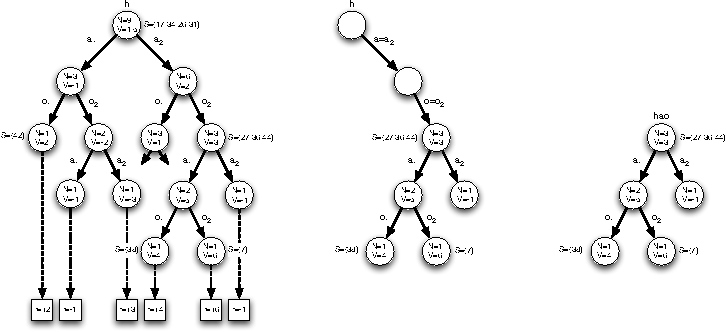
\includegraphics[width=1.0\textwidth]{figures/POMCP_original.pdf}
    \captionsetup{singlelinecheck=off}
    \caption[A POMCP belief tree]
    {
        A POMCP belief tree with two actions and two observations. The agent simulates action-observation trajectories starting from the current belief at history h (left). The action with the highest mean return from the simulations is executed in the real environment, and the agent receives a real observation o (middle). The tree can then be pruned, as all other histories are rendered invalid. The process repeats from the new history hao (right).
        \begin{flushright}\emph{Source: \cite{pomcp}}.\end{flushright}
    }
    \label{fig:pomcp_original}
\end{figure}

% The simulator is used to generate sequences of states, observations and rewards. These simulations are used to update the value function, without ever looking inside the black box describing the model’s dynamics.

POMCP constructs a search tree of histories (see figure \ref{fig:pomcp_original}). Sequences of states, observations, and rewards are simulated using a generative model. Given a state and action, the generative model returns a successor state, observation, and reward. The simulations allow POMCP to estimate the value of histories without knowing the exact transition dynamics of the POMDP. For each represented history, a node $T(h) = \langle N(h), V(h) \rangle$ is maintained. $N(h)$ stands for the number of times the history $h$ has been visited, while $V(h)$ stores the history's value. The value is estimated by the mean return from all searches that start at history~$h$. 

The belief over the states is approximated by employing an unweighted particle filter approach. The belief is represented by a collection of states. For every history $h$ visited during searches, the belief $B(h)$ is updated to include the simulation state (particle) returned by the generative model. The more likely a state is at a history, the more often it is expected to occur in simulations. As a consequence, the relative frequency of a state in the belief approximates its probability.

\begin{figure}[htbp]
    \centerfloat
    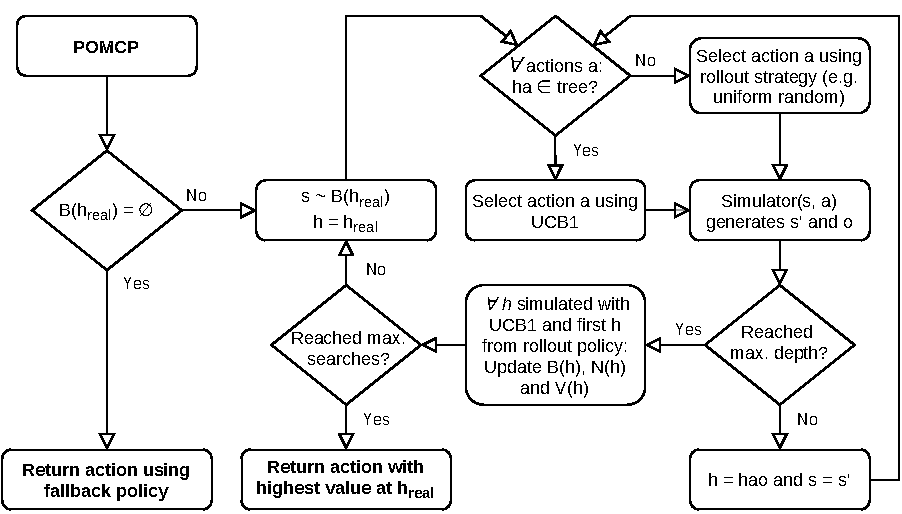
\includegraphics[width=1.0\textwidth]{figures/POMCP.pdf}
    \caption{Flow chart illustrating the \acrfull{pomcp} algorithm}
    \label{fig:pomcp}
\end{figure}

Figure \ref{fig:pomcp} illustrates the process of POMCP and Figure \ref{fig:pomcp-code} presents the pseudocode of the algorithm. If the belief for the current history $h_{real}$ does not contain particles at the beginning of a planning episode ($B(h_{real}) = \emptyset$), the agent has lost track of the environment's state completely. If this happens, we consider the planner to have failed and select actions randomly from this point on. Otherwise, a start state for a search is sampled from the belief at the current history: $ s \sim B(h_ {real})$. 

Searches are divided into two stages. During the first stage, which is active as long as child nodes exist for all children, actions are selected using the \acrfull{ucb1} algorithm \parencite{ucb1}. UCB1 chooses actions by the principle of optimism in the face of uncertainty; the values of actions are increased with an exploration bonus that is higher for rarely tried actions (see equation \ref{eq:ucb1}, $c$ is a constant hyperparameter). 

\begin{equation}
    V_{UCB1}(ha) = V(ha) + c\sqrt{\tfrac{log N(h)}{N(ha)}}
    \label{eq:ucb1}
\end{equation}

If any history is visited for the first time, the algorithm continues in the second stage: rollout. During this stage, the agent cannot rely on previous experiences to weigh the actions. Hence, actions are selected using a pre-defined rollout strategy $\pi_{rollout}$. We use uniformly random action selection during the rollout phase, if no preferred actions are applied (see section \ref{sec:preferred_actions}). First, all action nodes are initialized with initial counts $N_{init}$ and initial values $V_{init}$. These are usually zero unless preferred actions are
used.

Only for the first new history encountered during a rollout, a node is added to the tree. More histories may be simulated, but they are not included in the tree. The tree's growth is thereby limited to one level of depth per search. The main purpose of the rollout is to form a first estimation of the newly encountered history. After every search, the values at all nodes encountered during the search are updated by backpropagating the rewards through the tree.

To select which action to perform in the real environment, a fixed number of searches is performed from the current history. After all searches are complete, the action $a_{best}$ with the highest value at the current history $h_{real}$ is returned. After this action is executed in the real environment, with an observation $o_{last}$, the tree can be pruned. Only the nodes from history $h_{real}a_{best}o_{last}$ onward stay relevant as all other histories are rendered impossible (see figure \ref{fig:pomcp_original}). Then, the process repeats from the new history.

The number of searches performed during the planning has a substantial impact on the quality of the derived policy. Unfortunately, the computational complexity is exponential with respect to the number of performed searches. However, for a good policy, only a finite number of searches are required. The performance is expected to increase with the number of searches only until convergence occurs \parencite{pomcp}.

\begin{figure}[htbp]
    \centerfloat
    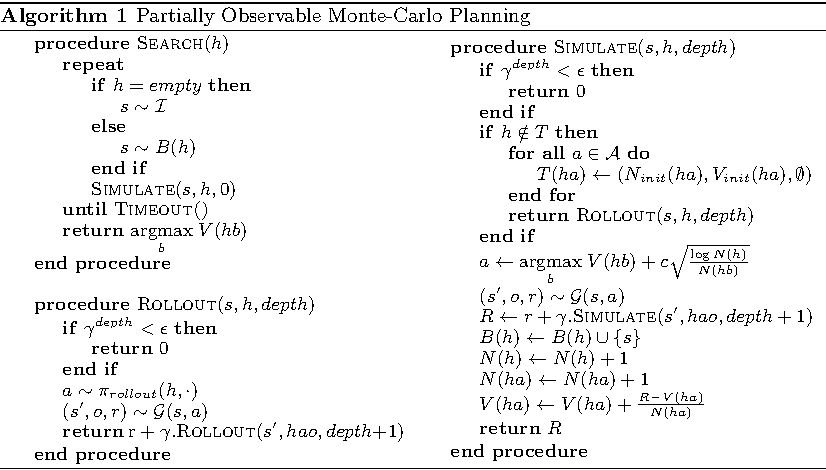
\includegraphics[width=1.0\textwidth]{figures/pomcp_alg_crop.pdf}
    \captionsetup{singlelinecheck=off}
    \caption[Original pseudocode for POMCP algorithm]
    {
        Pseudocode for the POMCP algorithm. \emph{Note: Instead of a time limit for the search procedure, we stop after a predefined number of searches have been performed.}
        \begin{flushright}\emph{Source: \cite{pomcp}}.\end{flushright}
    }
    \label{fig:pomcp-code}
\end{figure}

\subsection{Action and observation space discretization}
\label{sec:discretization}

\begin{figure}[htbp]
    \centering
    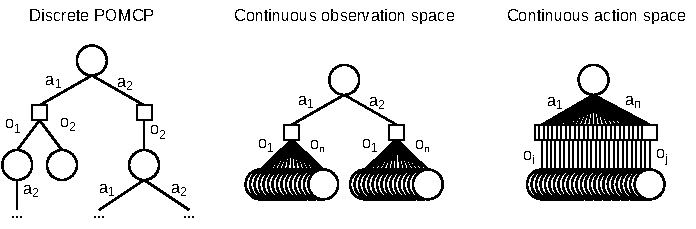
\includegraphics[width=1.0\textwidth]{figures/pomcp_continuous.pdf}
    \caption[Comparison of POMCP belief trees with discrete observations and continuous observations]{Comparison of POMCP belief trees with discrete observations (left) and continuous observations (right) with two actions.}
    \label{fig:pomcp_cont}
\end{figure}

POMCP is not suited to solve continuous POMDP. However, using POMCP with continuous states is possible as the particle filter approach can still provide a good approximation of the belief as long as the number of samples is large enough. The shared control lane-keeping task naturally has continuous actions and observations. To account for continuous action and observation spaces, discretization is necessary. Figure \ref{fig:pomcp_cont} shows how POMCP behaves when tasked with solving POMDP with continuous observation or action spaces without discretization. If the observations are continuous, the search tree cannot extend beyond the first observation layer as every observation is unique, and thus, no history will ever be visited twice. In the case of continuous actions, the chance of executing the same action twice is very low. Therefore, in this case, likewise, no history is reached twice. Planning becomes impossible. However, POMCP can be successfully applied with continuous POMDP by discretizing the action and observation spaces \parencite{pomcp_continuous}.

The action space is discretized as outlined before in section \ref{sec:actions} and the discretization of the observation space is defined in section \ref{sec:observations}. A balanced discretization resolution is chosen empirically. A too fine-grained discretization leads to very wide belief trees and can thereby hinder convergence. A coarse discretization increases the convergence probability but comes with a lower precision in planning.

\subsection{Particle deprivation and particle injection}
\label{sec:particle_deprivation}

Particle filter approaches, POMCP included, can fail due to a phenomenon called particle deprivation. Because of the random nature of the process, the belief sometimes converges towards a state that is far from the environment's true state. Particles that differ from the converged state have a low probability while sampling (low relative count). Hence, after every iteration, they become scarcer until they are completely erased from the belief. At this point, the agent is sure to be in an erroneous state and cannot recover anymore. Particle injection (also called particle reinvigoration) is a method to counteract this problem by introducing a number of random particles to the belief at each iteration \parencite{decision_making_book}. While this reduces the accuracy of the belief, it prevents its complete convergence towards a wrong state. 

Thus, particle injection is used to increase the variance of the belief about the driver model state. Figure \ref{fig:code-part-inj} showcases the pseudocode for our concrete implementation of particle injection. We sample states from the belief, transform them and inject the transformed states into the belief. 

The transformation only adapts the attentiveness of the driver and the number of remaining actions until the driver's attentiveness changes. The car state and the driver's last action stay unchanged. The attentiveness and the number of remaining actions (duration for the current state) are randomly chosen. The duration can be lower than the minimum defined in section~\ref{sec:driver_model} because the true remaining number of driver actions in a particular state might be lower after having performed actions already. Like in the original POMCP paper \parencite{pomcp}, the number of transformed particles added before each planning step is $1/16$ of the number of searches. The particles can be injected during policy execution, and therefore, do not influence the planning time.

\begin{figure}[htbp]
\lstset{basicstyle=\rmfamily\footnotesize,breaklines=true}
\begin{lstlisting}[mathescape=true]
$\textbf{procedure}$  $InjectParticles$()
    injections $\leftarrow$ 0
    $\textbf{repeat}$
        origState $\sim$ $B(h)$
        transformedState $\leftarrow$ $Copy$(origState)
        transformedState.driver.distracted $\leftarrow$ $Random$(true, false)
        transformedState.driver.duration $\leftarrow$ $Random$(0, maxDuration)
        $B(h)$ $\cup$ transformedState
        injections$++$
    $\textbf{until}$ injections == numSearches / 16
$\textbf{end procedure}$
\end{lstlisting}
\caption[Pseudocode for the particle injection]{Pseudocode for the particle injection. \emph{Note: Only the driver distraction and duration for the current state are changed in the transformed state. The car state and the driver's last action are copied.}}
\label{fig:code-part-inj}
\end{figure}


\subsection{Preferred actions}
\label{sec:preferred_actions}

\cite{pomcp} improve the performance of POMCP by providing domain knowledge in the form of preferred actions to the agent. Domain knowledge allows the agent to focus on promising states without altering the aglorithm's performance behavior \parencite{pomcp}. Preferred actions are initialized with an initial value $V_{init}$, increasing the likelihood to be selected by the UCB1 algorithm. Moreover, the rollout strategy $\pi_{rollout}$ can be changed from uniformly random action selection to a more informed method. Refer to figure \ref{fig:pomcp-code} to see how changing $V_{init}$ and $\pi_{rollout}$ integrates into the algorithm.

For example, \cite{pomcp} implemented preferred actions for the game Pac-Man, where the player is chased by ghosts in a maze who aim to catch and eat her. By collecting a \emph{power pill}, the player is enabled to eat the ghosts instead. When using preferred actions, the value of moving in directions in which the player sees ghosts is based on the power pill. If the player collected one, the value of moving towards ghosts is increased, if not, it is decreased. Thereby, the agent is made aware of basic domain knowledge, and its performance is increased.

In the case of the lane-keeping scenario on a highway, one thing to consider is that strong steering actions are seldomly needed. Strong actions should only be needed as a countermeasure when a distracted driver turns strongly in the wrong direction. The idea is to make minor actions more likely to be chosen during searches by giving them a higher initial value than stronger actions. Thereby, less-severe steering actions are selected and tried out first by the UCB1 algorithm. If they lead to good results, the agent can exploit them quicker. If not, the agent will also evaluate less preferred actions. 

We employ preferred actions to evaluate their effect on the performance of the agent. The design we use was empirically chosen and is not meant to provide a fully correct representation of driving domain knowledge. Instead of choosing actions uniformly random during rollouts, we use the probabilities shown in table \ref{tab:pref_actions} for the action selection by the rollout strategy $\pi_{rollout}$. Thereby, we favor minor steering actions over strong actions. The initial count $N_{init}$ is set to zero for all actions. The initial value for all actions is set to  $V_{init}$:

$$V_{init}(a) = 0.9 + 0.1 * Pr(a)$$

\begin{table}[htbp]
\footnotesize
\centering
\centerfloat
% \setlength{\tabcolsep}{3pt}
\begin{tabular}{@{}lcccccccc@{}}
\toprule
Action & $\pm$2 & $\pm$1     & $\pm$0.75  & $\pm$0.5   & $\pm$0.25  & $\pm$0.15  & $\pm$0.1   & 0 \\ \midrule
Probability (\%)  & 2.5   & 5 & 5 & 5 & 7.5   & 10 & 10 & 10 \\ \midrule 
Initial value  & 0.9025 & 0.905 & 0.905 & 0.905 & 0.9075   & 0.91 & 0.91 & 0.91 \\ \bottomrule
\end{tabular}
\caption[Preferred actions probabilities]{Preferred actions probabilities and initial values. The positive and negative values \emph{each} have the same probabilities and values.}
\label{tab:pref_actions}
\end{table} 